\chapter{Code du projet \textit{Calendar}}\label{code_calendar}

Voici le code Python du projet \textbf{Calendar}\footnote{Egalement disponible sur \textbf{Github} : \url{https://github.com/Krystof2so/PyCalendar}. Il se peut que sur le dépôt \textbf{Github} le code différe, le principe reste cependant le même, mais vous pouvez aussi utiliser l'exemple tel que fourni dans cette annexe} :

\begin{lstlisting}[style=python]
import calendar

from datetime import datetime
from PySide6.QtCore import QSize, Qt
from PySide6.QtWidgets import QApplication, QWidget, QVBoxLayout, QHBoxLayout,\
                              QGridLayout, QLabel, QPushButton
from PySide6.QtGui import QPalette, QColor


DAYS_OF_WEEK = ("Lundi", "Mardi", "Mercredi", "Jeudi", "Vendredi", "Samedi", "Dimanche")


class CalendarApp(QWidget):   
    def __init__(self):
        super().__init__()

        self.setWindowTitle("PyCalendar")
        self.setGeometry(100, 100, 400, 300)

         # Initialiser la date actuelle :
        self.current_date = datetime.now()

        # Layout vertical principal :
        main_layout = QVBoxLayout()
        self.setLayout(main_layout)

        # Layout horizontal pour afficher le mois en cours et les boutons de navigation:
        month_layout = QHBoxLayout()
        main_layout.addLayout(month_layout)

        # Bouton pour le mois précédent :
        self.prev_button = QPushButton("<")
        self.prev_button.setFixedSize(QSize(30, 30))  # Définir une taille fixe pour le bouton
        self.prev_button.clicked.connect(self.show_previous_month)
        month_layout.addWidget(self.prev_button)

        # QLabel pour afficher le mois en cours :
        self.month_label = QLabel(self.get_current_month_year())
        self.month_label.setAlignment(Qt.AlignCenter)
        month_layout.addWidget(self.month_label)

        # Bouton pour le mois suivant :
        self.next_button = QPushButton(">")
        self.next_button.setFixedSize(QSize(30, 30))  # Définir une taille fixe pour le bouton
        self.next_button.clicked.connect(self.show_next_month)
        month_layout.addWidget(self.next_button)

        # Ajouter la grille du calendrier :
        self.calendar_layout = QGridLayout()
        main_layout.addLayout(self.calendar_layout)

        # Remplir la grille avec les jours du mois :
        self.populate_calendar()

    def get_current_month_year(self):
        return self.current_date.strftime("%B %Y")

    def is_today(self, day):
        """Vérifie si le jour donné est aujourd'hui."""
        today = datetime.now()
        return day == today.day and self.current_date.month == today.month and self.current_date.year == today.year

    def populate_calendar(self):
        """Obtenir les jours du mois, et les placer dans la grille."""
        year = self.current_date.year
        month = self.current_date.month
        cal = calendar.monthcalendar(year, month)
        # Effacer la grille précédente :
        self.clear_layout(self.calendar_layout)
        # Ajouter les jours de la semaine :
        for col, day_label in enumerate(DAYS_OF_WEEK):
            label = QLabel(day_label[0:2])
            label.setAlignment(Qt.AlignCenter)
            self.calendar_layout.addWidget(label, 0, col)
        # Ajouter les jours du mois :
        for row, week in enumerate(cal):
            for col, day in enumerate(week):
                label = QLabel("" if day == 0 else str(day))
                label.setAlignment(Qt.AlignCenter)
                if self.is_today(day):
                    palette = label.palette()
                    palette.setColor(QPalette.WindowText, QColor('#A3BE8C'))  # Vert du thème Nord
                    label.setPalette(palette)
                self.calendar_layout.addWidget(label, row + 1, col)

    def clear_layout(self, layout):
        """Effacer tous les widgets d'un layout."""
        while layout.count():
            child = layout.takeAt(0)
            if child.widget():
                child.widget().deleteLater()

    def show_previous_month(self):
        """Afficher le mois précédent."""
        if self.current_date.month == 1:
            self.current_date = self.current_date.replace(year=self.current_date.year - 1, month=12)
        else:
            self.current_date = self.current_date.replace(month=self.current_date.month - 1)
        self.month_label.setText(self.get_current_month_year())
        self.populate_calendar()

    def show_next_month(self):
        """Afficher le mois suivant."""
        if self.current_date.month == 12:
            self.current_date = self.current_date.replace(year=self.current_date.year + 1, month=1)
        else:
            self.current_date = self.current_date.replace(month=self.current_date.month + 1)
        self.month_label.setText(self.get_current_month_year())
        self.populate_calendar()

if __name__ == "__main__":
    app = QApplication([])
    window = CalendarApp()
    window.show()
    app.exec()
\end{lstlisting}

Voici une image de ce que ce code propose :
\begin{figure}[h!]
    \centering
    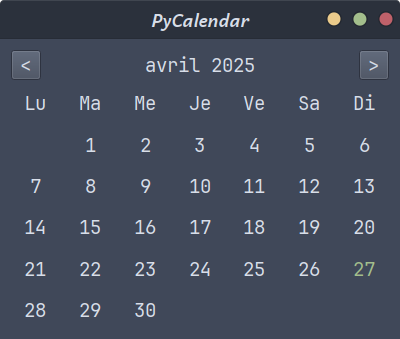
\includegraphics[width=0.6\textwidth]{IMG/PyCalendar.png}
    \caption{Application \textbf{Calendar}}
\end{figure}

L'arborescence du projet est la suivante :
\begin{lstlisting}[style=tree]
Calendar
|\textbar|-- IMG
|\textbar|   |\textbar|-- PyCalendar.png
|\textbar|-- README.md
|\textbar|-- src
    |\textbar|-- pycalendar
        |\textbar|-- main.py
\end{lstlisting}
